\section{Fundamentals of astronomical observation} \label{intro}
\subsection{Basics of CCD detectors} \label{ccd}
Instead of photographic plates like in the beginning of photography, people now widely use \textit{Charged coupled devices} (CCDs) for the detection of optical radiation, in visible light cameras and in modern telescopes. The working principle of CCD is as follows: Electrons produced by photoelectric effect are collected in the potential walls of the capacitors on a two-dimensional array of pixels made of semiconductors capacitors. The collected charges are first read out by being shifted column by column and sent to counting device (output register) at the end of each horizontal line, which consists of a series of electrodes. Then the signal is amplified and an offset, also called bias, is added so it can be digitalized by an \textit{Analogue digital converter} (ADC). The offset is required to ensure all values are positive since the ADC can only handle values greater then zero.  After calibrating and analysing numerical data one can reconstruct the distribution of observed astronomical objects. \\
\begin{figure}[h]
	\begin{subfigure}{0.5\textwidth}
	\centering
	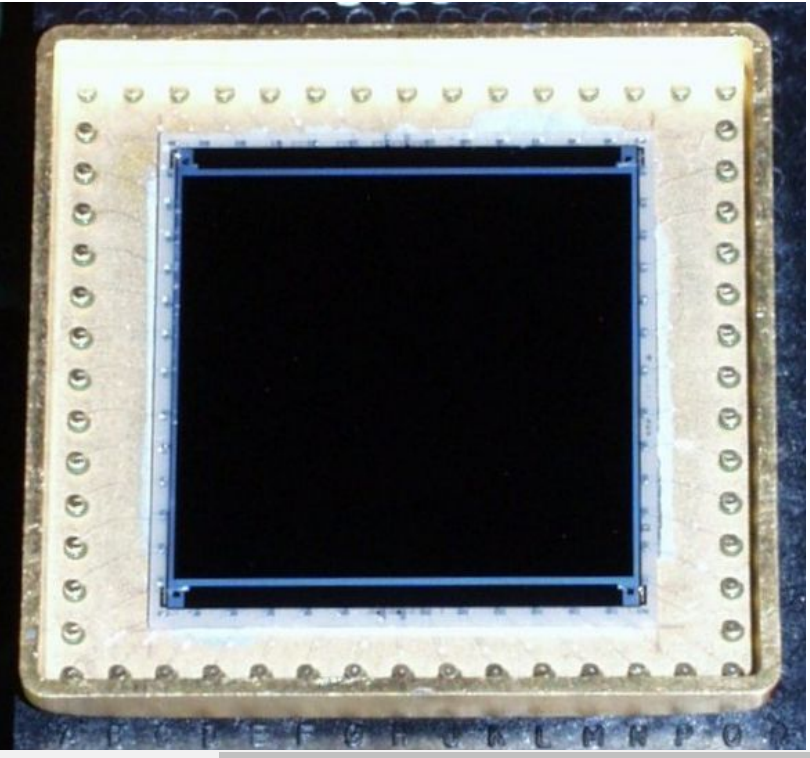
\includegraphics[width=0.9\linewidth ,height=7cm]{report_pictures/CCD.png}
	\caption{A CCD detector}
	\label{CCD}
	\end{subfigure}
	\begin{subfigure}{0.5\textwidth}
	\centering
	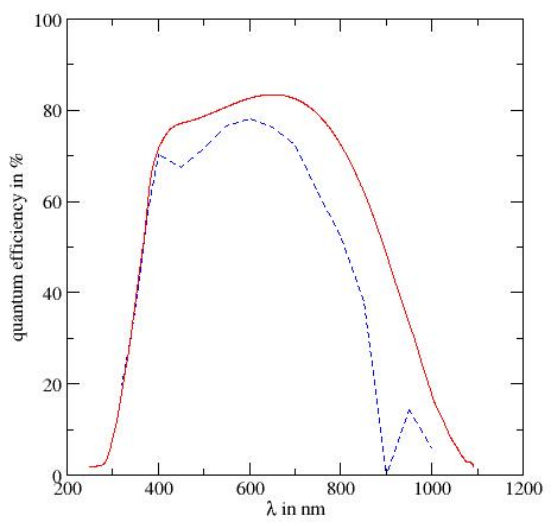
\includegraphics[width=0.9\linewidth ,height=7cm]{report_pictures/QE.png}
	\caption{Quantum Efficiency }
	\label{QE}
	\end{subfigure}
	\caption{Examples taken from the Manual \cite{manual}}
	\label{examples}
\end{figure}
\subsubsection{Advantages of CCD detectors}

Some of the numerous perks the CCD offers, besides delivering the data in digital form, are:
\begin{itemize}
\item {\textbf{Good spatial resolution:}}
The resolution and the field of an image taken by a CCD depend on its number of pixels. With large amount of pixels in small volume of CCDs one can see the details at the surface of the studied object.
 

\item\textbf{Very high quantum efficiency over large spectral window:}
CCDs are sensitive to the radiation in a large wavelength domain. The fraction of detected photons on CCD reaches more than 50\% ($>$ 80\% at certain wavelengths), which enables the detection of very faint objects. 

\item\textbf{Very good linearity:}
There exists good linear relation between measured signal and incoming photon flux, which is proportional to the exposure time, with a large saturation threshold and no requirement on minimum exposure time. CCDs are linear to an accuracy of about 0.1\% within their dynamical range.
  
\item{\textbf{High photometric precision and a reliable rigidity:}}
Since CCDs are made of solid elements and the position of each pixel is fixed in a rigid way during the production, there's usually no physical distortion and the sensitivity of CCDs is stable in time.  

\item\textbf{High dynamic range:}
The brightest object that can be detected depends on the capacity of pixels to collect photoelectrons before they saturate, which increases with the individual pixel. The faintest object that can be detected are determined by the signal to noise ratio. The dynamic range represents the maximum possible ratio between the fluxes of the faintest objects and the brightest ones, which is small for CCDs, so that people can detect objects with high difference in magnitudes at the same time.
\end{itemize}
In this experiment we will confirm the linearity of our CCD and analyse different noise sources.
\hspace{4mm}
\subsubsection{Noise sources of CCD detectors}\label{noise}
We will specifically look at three different noise sources when observing a flat illuminated surface:
\begin{itemize}
\item\textbf{Read-out Noise $\sigma_{r}$:}
The read-out noise originates from the gate amplifier and doesn't scale with the number of incoming or detected photons. This error can be measured by looking at a difference image of two 0 milliseconds exposure time images \cite{readout} or measuring the scatter of the bias, which is what we will do. The bias will be recorded in each picture as a 26 pixel extension of our image at the right edge.

\item\textbf{Photon Noise $\sigma_{ph}$:}
Incoming Photons are subject to fluctuations which can be described with Poisson statistics, meaning the amount of measured Photons of a uniformly lit area can vary with $\sqrt{N_{ph}}$. Further we have to consider the quantum efficiency and the fact, that the final picture we can see is acquired through an ADC, which counts $\kappa$ electrons as one \textit{count}. This all leads to a formula for the photon noise as follows:
\begin{equation}\label{sig_phd}
	\sigma_{ph,d}^2 = \dfrac{\eta}{\kappa} N_{ph,d}.
\end{equation}
Where $N_{ph,d}$ will be the median of the \textit{counts} in the image.

\item\textbf{Pixel response non uniformity Noise $\sigma_{PRNU}$}:
Each pixel has a slightly varying quantum efficiency, resulting in a noise which scales directly with the incoming photon number. It scales linear with photon number compared to the square root dependency of $\sigma_{ph}$. The scaling factor is of the order $10^{-2}$. Resulting from those dependencies we expect $\sigma_{PRNU}$ to dominate for high signals and $\sigma_{ph}$ for the lower ones. Since the pixel difference is a characteristic of each pixel, it generally should be the same for images taken with the same exposure time of the same objects.
\end{itemize} 
If we now consider those noise sources we can write the total noise of the image as follows:
\begin{equation}\label{sig_tot}
	\sigma_{tot,d}^2 = \sigma_{PRNU,d}^2 + \sigma_{ph,d}^2 + \sigma_{r,d}^2 .
\end{equation}
As mentioned above we will be able to determine the read-out noise directly from the image by taking the standard deviation in the overscan region. But the other 2 noise sources are not as easily accessible since even with the approximation of $\eta = 1$ we still are missing our gain and we don't know the exact scaling factor for our \textit{prnu} noise. For that we will utilize the characteristic of $\sigma_{PRNU}$ being the same for observation of the same object with same exposure time. If we record two images in sequence and subtracts each pixel value we acquire the so-called \textit{difference image}. It will consist only of the other 2 noise sources, since we removed the initial signal as well as the $\sigma_{PRNU}$. We can express the scatter of that image as follows:
\begin{equation}\label{diff_img}
	\sigma_{diff,d}^2 = 2(\sigma_{ph,d}^2 + \sigma_{r,d}^2)
\end{equation}
From eq \eqref{diff_img} and eq \eqref{sig_tot} we can now determine $\sigma_{ph,d}$ and $\sigma_{PRNU}$.
\hspace{4mm}
\subsection{Basics of astronomical data} \label{astrodata}
Besides the noise we looked at there are several other physical effects one has to take into consideration when analysing the image.

\subsubsection{Data-influencing effects}
Some effects influence data quality and there are different methods to deal with them:

\begin{itemize}

\item\textbf{Noise and dynamic range:}
Despite of large dynamic range of CCDs it is not always possible to simultaneously assure a good signal to noise ratio for weak objects of interest, while not saturating very bright stars. Thus it is important to select exposure time carefully depending on the purpose of the observation.

\item\textbf{Extrema of data:}
A certain amount of pixels on the detector are "dead", i.e. produce no physically significant signal at all. The amount and distribution of these pixels stays the same over time. Additionally some other pixels are activated by cosmic rays such as electrons, $\gamma$-rays, muons, etc. Around the impact position the pixels are saturated or show high numbers of counts. The distribution of these pixels is random and the number of them depends on integration time. To get rid of these extrema people use method called \textit{dithering} or \textit{jittering} by taking several exposures (at least 5) with the telescope being moved slightly between each exposure. The multiple frames are then aligned and the median of each pixel of the combined image is determined. With this method the signal to noise ratio is also improved without saturating brighter sources.

\item\textbf{Diffraction by aperture:}
Light is diffracted when passing through apertures, the diffraction effects increase with decreasing aperture size. The degree of spreading (blurring) of a point object is a measure for the quality of an imaging systems, which is described with a \textit{Point spread function} (PSF). For a diffraction-limited optical system operating in the absence of aberrations, i.e. a perfect lens with a uniformly illuminated circular aperture, the PSF is the Airy disc, a bright central region surrounded by concentric rings. In astronomy the Airy disc is used to determine the quality and alignment of the optical components of a telescope. The Rayleigh criterion for barely resolving two objects is that the centre of the Airy disc for the first object occurs at the first minimum of the Airy disc of the second.

\end{itemize}

\subsubsection{Data reduction}\label{reduction}
The previously described effects and corresponding methods don't include any alteration of the taken data. Other effects can be treated right away without consideration of the observed objects. Those effects can be negated through altering the data in certain ways. The ones which we will take a closer look in this experiment are:
\begin{itemize}
\item\textbf{Bias:}
The previously mentioned offset, the bias, added to prevent malfunctioning of the ADC has to be determined and subtracted. As also mentioned above we will determine it from a small border region in our images called the \textit{overscan region}. The bias will be determined for each picture separately and subtracted.

\item\textbf{Dark current:}
Dark current refers to the signal produced through the thermal energy of the electrons in the CCD. It leads to a detected signal even if no photons are reaching the CCD. It depends on the temperature as follows:
\begin{equation}\label{dark_current}
	I_{dark} = \textit{const } T^{\frac{3}{2}} e^{- \frac{E_g}{k_b T}}.	
\end{equation} \\
$E_g$ is the bandgap of the material in the detector, which is silicone in our case, T is the temperature and $k_b$ is the Boltzmann constant. We will measure the temperature dependency of the dark current by taking images with the shutter closed, i.e. no photons will be detected, while the CCD is getting cooled down. Since the measured \textit{counts} are proportional to the current measured, which with no detectable photons is only the dark current, we can verify the eq \eqref{dark_current} as well as determine the bandgap of silicone. If the dark current value is not negligible at the working temperature, one would have to subtract it from every image as well.

\item\textbf{Flat fields:}
Different sensitivity of each pixels due to imperfect production of the CCD results in small scale variations. On the other hand, there exists large scale variations caused by the optics (\textit{vignetting}) and contaminations in the optical path. These variations, causing difficulties in comparing objects from different region, are however constant at least during the observation. For corrections one exposes the whole detector to a structureless and homogeneously emitting surface, i.e. flat field, and records the variations. In practice the flat field is provided either by a white surface hanging on the inner side of the dome or the twilight sky. Though the twilight period is rather short, the sky-flatfield provides the same condition as real observation and is thus preferred. For the data reduction purpose one has to take multiple images and take median value for each pixel to create a master flat-field. Then you normalize the master flat-field with its median to produce a \textit{relative image matrix} which contains the relative strength of each pixel to each other. Every measurement frame is then later divided by that normalized master frame. Each filter requires its own master frame since the optical set up is changed.

\end{itemize}

\subsection{Basics of photometry} \label{photometry}
With CCD detectors one can measure the radiation flux or intensity of an astronomical object reaching the earth. This process, photometry, uses the unit of magnitudes and is essential to understanding stars and other astronomical subjects. 

\subsubsection{Magnitudes}
The luminosity of a star $L$ is defined as emitted energy per unit time. The flux reaching an observer in a distance $d$ is given by $F=\frac{L}{4\pi d^4}$. The intensity is defined as flux per solid angle. One can differentiate between several different magnitudes:
\hspace{3mm}
\begin{itemize}
\item\textbf{Instrumental magnitude:}
For measurements by the same instruments and under similar conditions, the comparison of different sources is realised by instrumental magnitudes. The measured counts are converted to a logarithmic scale with arbitrary zero point: 
\begin{equation}
\label{instrumental}
	m_{instr.} = zero point -2.5 \log_{10} {(counts)}
\end{equation}
The counts is calculated either by simply summing over an aperture centered on the star, i.e. aperture photometry, or by fitting a PSF to the profile of the star, i.e. PSF photometry.

\item\textbf{Apparent magnitude:}
The brightness of stars perceived from earth, the apparent magnitude, was once classified by eye ranging from 1 for the brightest stars to 6 for barely visible stars. It was later quantified assuming a logarithmic perception. For the flux of two stars it means:
\begin{equation}
\label{Flux}
	\frac{F_2}{F_1}=100^{(m_1-m_2)/5}
\end{equation}
With the help of standard stars the difference between instrumental magnitude and apparent magnitude is determined and observed magnitude is then calibrated. The effects of different instruments and circumstances for comparison of magnitudes are hence eliminated.

\item\textbf{Absolute magnitude:}
To compare objects in different distance one can use the absolute magnitude, which is the apparent magnitude $M$ of an object if it were in distance of 10 pc from our sun. The relation between apparent and absolute magnitude satisfies 
\begin{equation}
\label{AppAbs}
	\frac{F_{in 10 pc}}{F}=(\frac{d}{10 pc})^2=100^{(m-M)/5}
\end{equation}
with $d$ as the distance between the star and the observer in pc.However $d$ is usually unknown which makes it hard to compare stars absolute magnitude. One could calculate the distance of an object with absolute and apparent magnitude as follows
\begin{equation}
	d = 10^{\dfrac{m-M+5}{5}}.
\end{equation} 
The expression $m-M$ is called the distance modulus. 

From the absolute magnitude of a star at the same distance as a reference star with known luminosity and absolute magnitude, it's possible to determine its luminosity:
\begin{equation}
\label{Lumi}
	\frac{F_2}{F_1}=\frac{L_2}{L_1}=100^{(M_1-M_2)/5}
\end{equation}

\item\textbf{Bolometric magnitude:}
The Bolometric magnitudes  $M_{bol}$ corresponds to the flux integrated over all wavelengths. Its direct measurements are only possible by space observatories. From earthbound observations people have only theoretical estimate because of detector limitations and atmosphere's absorption of certain wavelength. Alternatively a wavelength dependent magnitude $M_{\gamma}$ for luminosity in a certain wavelength range is used.
\end{itemize}

\subsubsection{Observation of a star}
Through observation people want to learn physical properties of a star. The flux is related to star's surface temperature, given by Stefan-Boltzmann law: $F=\sigma T_{eff}^4$ with $\sigma = 5.67\times10^{-8}$ Wm$^{-2}$K$^{-4}$ Stefan-Boltzmann constant and $T_{eff}$ being the temperature of a black body emitting the same radiation power. Furthermore people are also interested in the mass of a star and its metallicity, from which its evolution can be deduced. In astronomy all the elements besides H, He and their isotopes are called metals which for a star is referred to as its metallicity. It is however not trivial to calculate the mass of a star from easily accessible observables.
\hspace{4mm}\\
\subsection{Basics of spectroscopy}
Spectroscopy is the measurement of the special intensity of the emitted light with high accuracy. But since the CCD image doesn't contain any direct information about color we use filters to extract those information out of multiple images. \\
Filters that transmit a certain part of the spectrum are used to obtain rough spectral information. A common used filter system is Johnson filter system with broad band filters, which contain U(ultraviolet), B(blue), V(visual, i.e. green), R(red) and I(infrared) filters.\\
To quantify spectral properties color index is defined as difference between magnitudes with different filters:
\begin{equation}
 m_B-m_V=M_B-M_V=B-V.
\end{equation}
The special characteristic of this color index is the invariance of the number. It is the same for  apparent magnitude and absolute magnitude. It further gives information about the temperature of the star since the index gives us information about the spectrum of the star which we can connect to a temperature by looking at black body radiation spectrum. We will call the apparent magnitude of a certain Johnson filter with the letter given above.\\
To compare measurements with different filter systems a calibration with standard stars is applied. Assuming the transmission curve for the B filter is slightly different, the calibration of the instrumental magnitude can be calculated in a first order approach.
\hspace{4mm}

\subsection{Relevant astronomy}
With the magnitudes of those stars and corresponding color index we can now relate those to each other to find out more. But first we will introduce globular clusters.\\
\subsubsection{Globular clusters}
Globular clusters, spherically collection of stars, are by now counted to the oldest objects found in the universe. The stars in a globular clusters in our milky way are very metal poor, which indicates their formation in early stage of the universe when the interstellar matter was not enriched with heavier elements than hydrogen and helium. With about 150 globular clusters known, the distribution, velocity and composition of globular clusters provide information about the evolution of our galaxy. The age identification of globular cluster shows however large errors and discrepancies with different measurements.
\hspace{2mm}
\subsubsection{The Hertzsprung-Russel-Diagram}
At the beginning of last century, Hertzsprung and Russel used data of  photometrically measured stars, independently discovered the correlation between the spectral type, effective temperature and luminosity, as shown in Hertzsprung-Russel-Diagram (HRD). An example is of an HDR is shown in figure \ref{HRD}. The majority of the visible stars experiencing the phase of hydrogen burning locate in the \textit{main sequence} diagonal region. Different regions in the diagram indicate different masses, distances, evolution phases of stars. For example, O stars refers to young, massive and luminous objects.

\begin{figure}[h]
	\begin{subfigure}{0.5\textwidth}
	\centering
	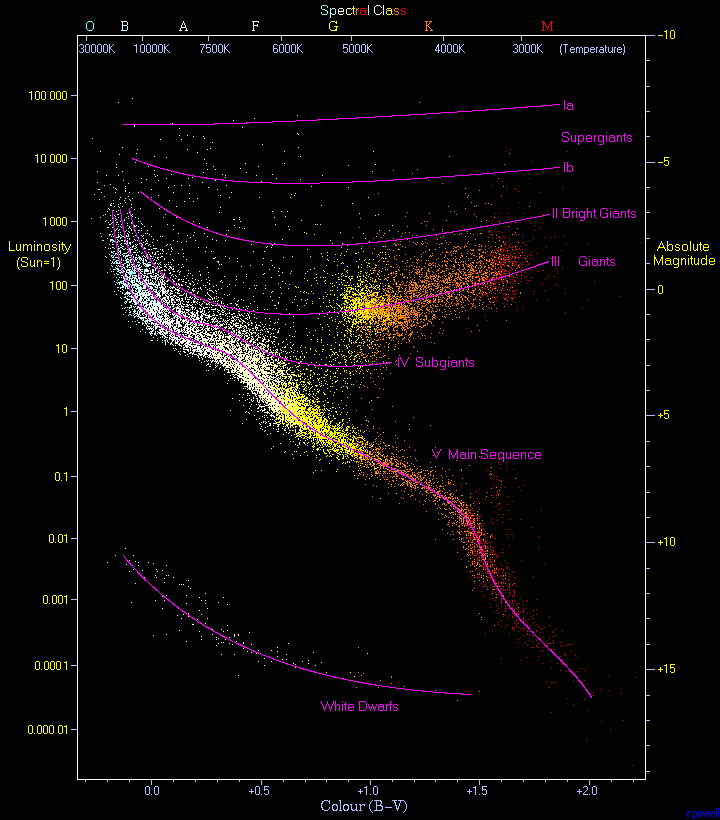
\includegraphics[width=0.9\linewidth ,height=10cm]{report_pictures/HRDiagram.png}
	\caption{Hertzsprung-Russel Diagramm \cite{HRWiki}}
	\label{HRD}
	\end{subfigure}
	\begin{subfigure}{0.5\textwidth}
	\centering
	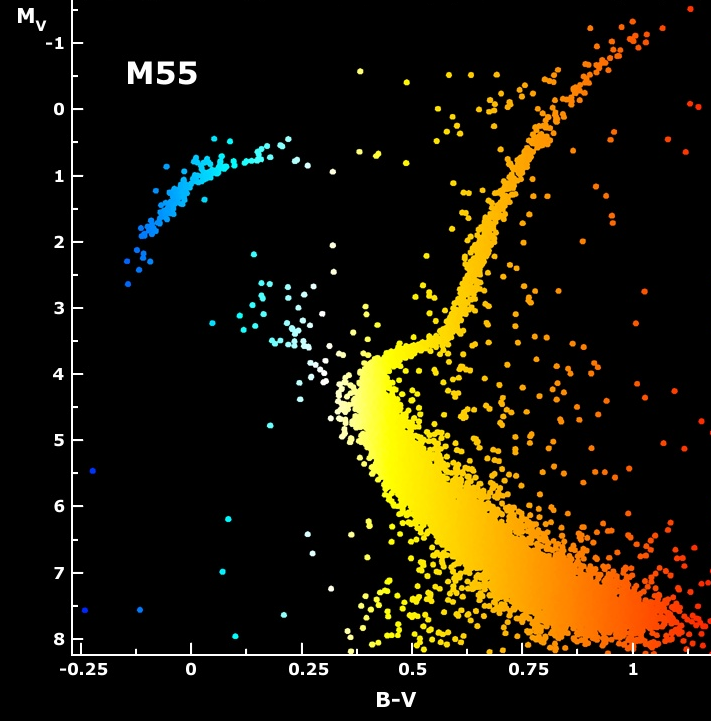
\includegraphics[width=0.9\linewidth ,height=8cm]{report_pictures/CMDiagram.png}
	\caption{Color-magnitude Diagram \cite{NASA}}
	\label{GC_ex}
	\end{subfigure}
	\caption{Example of the different diagrams}
	\label{diagram}
\end{figure}

\subsubsection{Color-Magnitude-Diagram}
In practice it is often difficult to produce a HRD, instead a Color-Magnitude-Diagram (CMD) plotted with the apparent magnitude against a related color index, determined directly from observations with two filters, is used. A CMD provides also large amounts of important information as a HRD.
Globular Clusters are well suited for the analysis with a CMD, since all their stars are located at the approximate same distance and have the same metallicity. This leads to an easy approximation of the distance modulus The CMD of a globular cluster has a characteristic form as seen in figure \ref{GC_ex}.
\hspace{4mm}
\subsubsection{Analysis with a CMD}
Assuming all stars within the cluster have similar ages, one can read off the age of the cluster from the CMD. Since massive and luminous at the top left end of the CMD burnt their hydrogen in their cores within short lifetime and turned into a red giant, the older a cluster is, the lower mass stars move from main sequence into the red giant branch. The shifts to stars with lower mass and luminosities, i.e. turn off point, whose position depends also on metallicity of the cluster, are good indicators for age of older clusters. For young clusters there may exists ambiguity. 
\vspace{3mm} \\
Since in a globular clusters one can approximate, that the stars are at the same distance with same chemical composition as well as similar ages one can read the distance to cluster from a CMD. The position of the main sequence is compared to the position of a cluster with known distance. With some presumptions ignoring effects of different matallicities and of attenuation by interstellar dust, the distance modulus of the cluster can be deduced by the shifts. Alternatively it can be compared to predictions of its position by theoretical models, for example \textit{isochrones}, i.e. curve representing stars of the same age. 
\vspace{10mm}